\chapter{nHCal}\label{cha:nHCal} % chktex 24
extensively from pre-TDR - new iteration in two weeks - is it worth the wait?

WHERE IS THE GOOGLE DOC? 

Overview from some Leszek's presentation? is Leszek relevant?

\section{Motivation}
still tail catcher of nECal (what is that really, only of that?)

start with HERA (maybe) - then continue from that ("to not make the same mistake")

Vector meson - the matrix image + the 012K plots

only for e + Au and phi, or also e + p, and J/psi?

\section{Construction}
realistic dimensions and location

tiling? is it really important?

does clustering make sense to mention? - probably somewhere else (simulations)

changes?:

sampling, N layers, ... ok, but what about material e.g.?

sampling fraction - possible to be compensating (Elke says NO)? what did Subhadip prove, then? - how achieved? how calculated?

but what about true construction? does Leszek now? does anybody?

two images from BP? or something else? cite myself?

anything about neutrons? meaningful?

\section{?}
is tilt usable? if for VU, also for DP?

forgot about material plot!!

\section{answers}

MATERIAL:
really non-magnetic steel

\pagebreak

\begin{figure}[H]
    \centering
    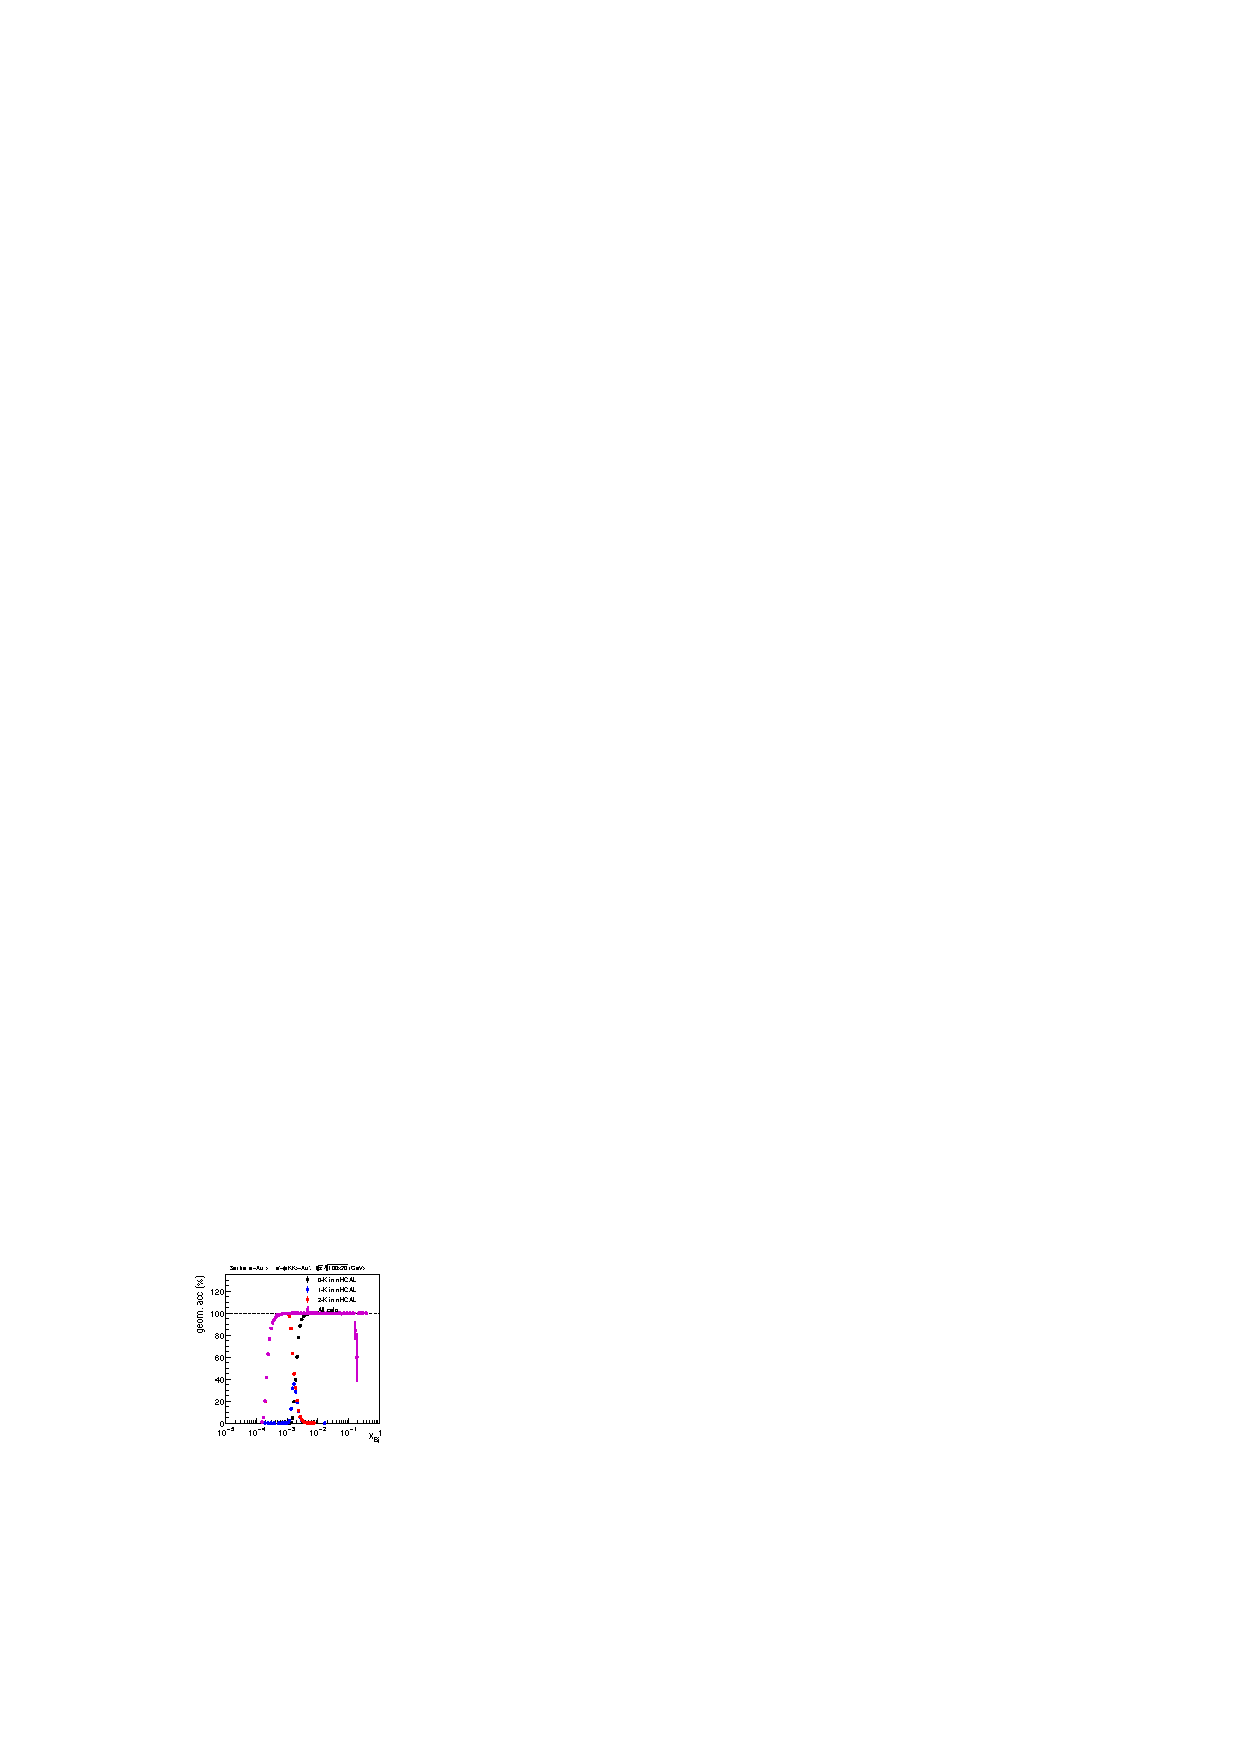
\includegraphics[width=.7\linewidth]{img/e+Au-phi(KK).pdf}
    \caption{[Caroline paper]}
    \label{fig:nhcal:e+Au-phi(KK)}
\end{figure}

\begin{figure}[H]
    \centering
    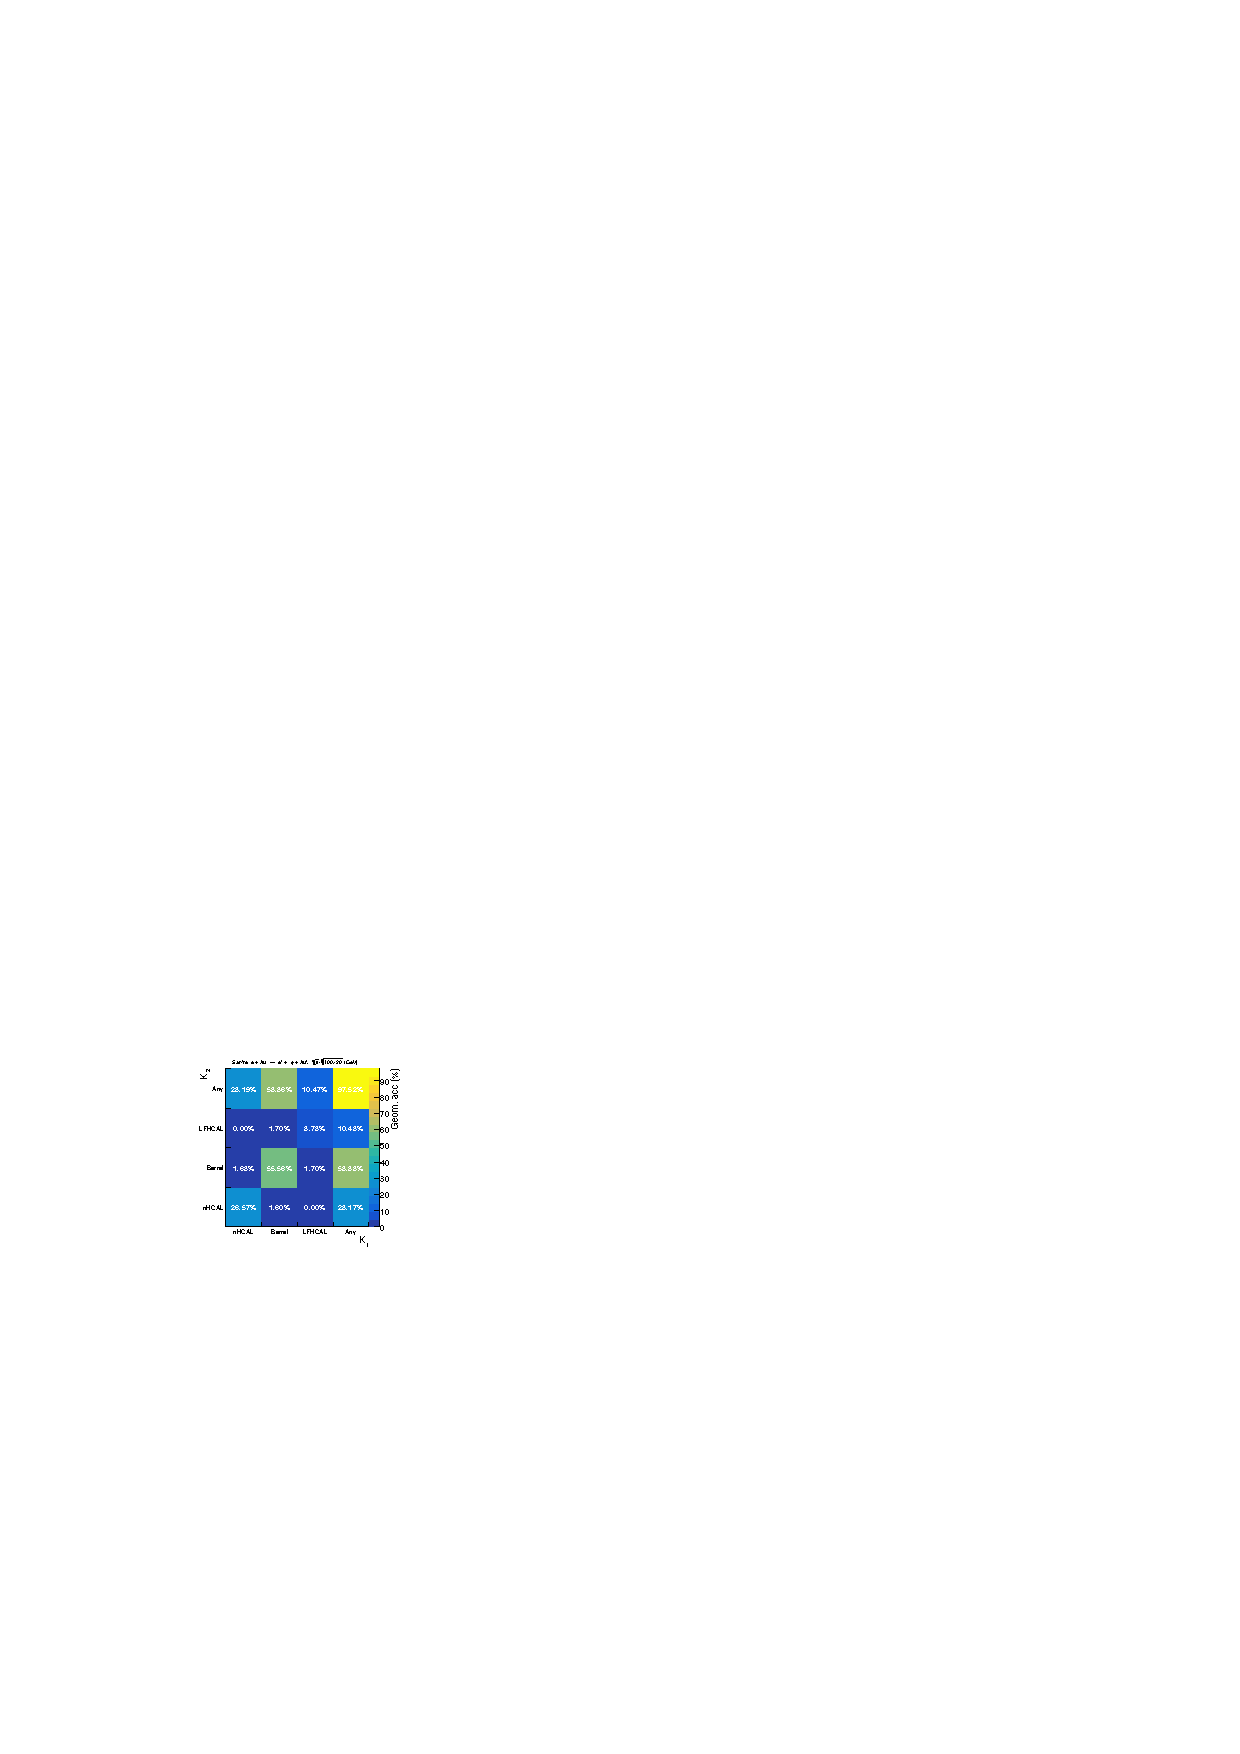
\includegraphics[width=.7\linewidth]{img/K1K2matica.pdf}
    \caption{[Caroline paper]}
    \label{fig:nhcal:K1K2matica}
\end{figure}
